\newpage
\hypertarget{remCard vis}{}
\subsection{Partition::removeCard(Card) - The visual syntax}
\visHeader

\begin{itemize}

\item[$\blacktriangleright$] In Enterprise Architect (EA), open the main diagram in Enterprise Architect (EA) from Eclipse by double-clicking the \texttt{.eap}
file, and carefully do the following: (1) Click \emph{once} on \texttt{Partition} to select it, then (2) Click \emph{once} on the method
\texttt{removeCard} to choose it (Fig.~\ref{fig:sdm_start}). (3) \emph{Double-click} on the chosen method to indicate that you want to implement it.

\begin{figure}[htp]
\begin{center}
  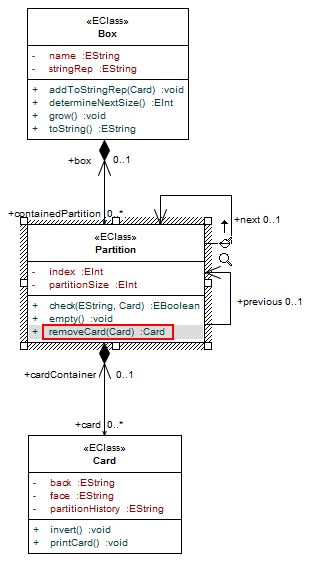
\includegraphics[width=0.6\textwidth]{ea_startSDM}
  \caption{Double-click a method to implement it}  
  \label{fig:sdm_start}
\end{center}
\end{figure}
 
\item[$\blacktriangleright$] If you did everything right, a new \emph{activity diagram} should be created and open in a new tab with a cute little \emph{start node} 
labelled with the signature of the method (Fig.~\ref{fig:sdm_skeleton}).  

\begin{figure}[htp]
\begin{center}
  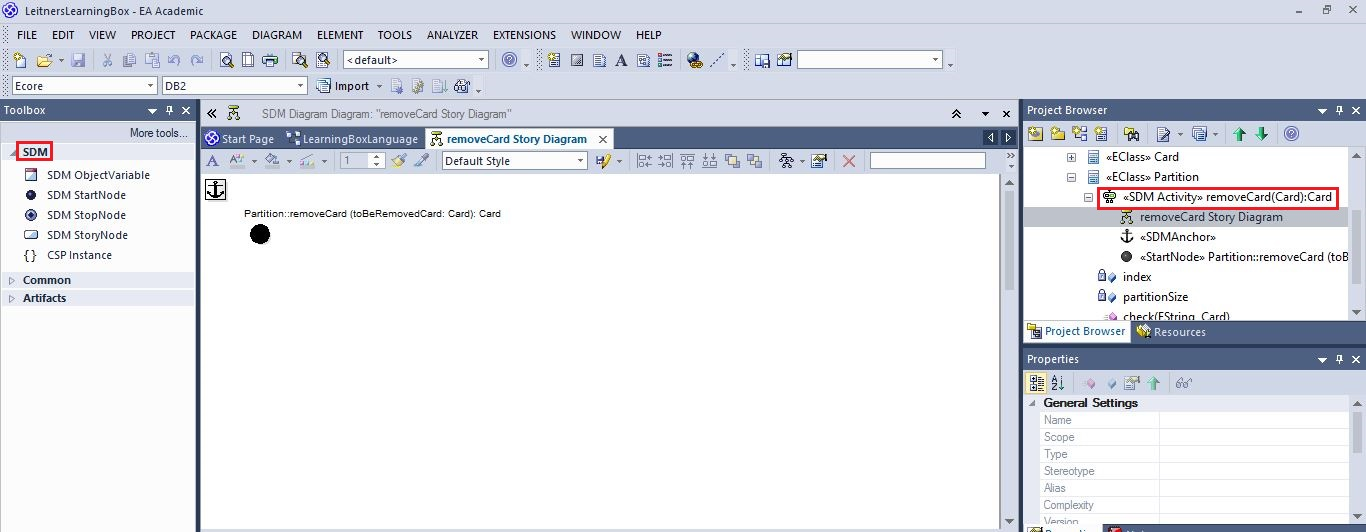
\includegraphics[width=1.0\textwidth]{ea_generatedSDM}
  \caption{Generated SDM diagram and start node}  
  \label{fig:sdm_skeleton}
\end{center}
\end{figure}

\vspace{0.5cm}

\item[$\blacktriangleright$] Let's quickly get familiar with the EA workspace. First, inspect the project browser and notice that an \texttt{<<SDM Activity>>}
container has been created for the method \texttt{removeCard} to contain this new \emph{activity}. If you're at any time unhappy with an SDM,\footnote{As you
might have already noticed, we use ``SDM'' interchangeably to mean our graph transformation language \emph{or} a concrete transformation (a story model) used
to implement a method and consisting of an activity diagram and a pattern in each story node.} you can always delete the appropriate container in the project
browser and start from scratch. This container will eventually host every diagram related to this pattern.

\vspace{0.5cm}

\item[$\blacktriangleright$] Next, note the new \texttt{SDM} toolbox that has been automatically opened up for the diagram and placed to the left above
the common toolbox. This provides quick access to common SDM items that you can use in your diagram.

\vspace{0.5cm}

\item[$\blacktriangleright$] Finally, in the top left corner of the diagram, you'll notice a small anchor. Double click on this icon to quickly jump back to the
metamodel. From there, double click the method again to jump back to the SDM. This is just a small trick to help you shift between diagrams quickly. 

\vspace{0.5cm}

\item[$\blacktriangleright$] To begin, choose the start node, and note the small black arrow that appears (Fig.~\ref{fig:sdm_quicklink}). 

\newpage

\begin{figure}[htp]
\begin{center}
  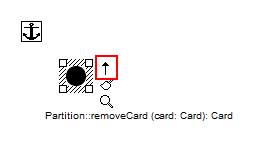
\includegraphics[width=0.5\textwidth]{ea_sdmStartNode}
  \caption{Quick link in SDM diagram to create new activity node}  
  \label{fig:sdm_quicklink}
\end{center}
\end{figure}

\item[$\blacktriangleright$] Similar to quick linking\footnote{Refer to Part II, Section 2.5}, a second fundamental gesture in EA is \emph{Quick Create}. To
quick-create an element, pull the arrow and click on an empty spot in the diagram. This is basically ``quick linking'' to a non-existent element.

\item[$\blacktriangleright$] EA notices that there is nothing to quick-link to, and pops up a small context-sensitive dialogue to create an element that can be
connected to the indicated source element.

\item[$\blacktriangleright$] As illustrated in Fig.~\ref{fig:sdm_new_activity_node}, choose \texttt{Append StoryNode} to create an \emph{activity
node}. We refer to the whole activity diagram simply as the \emph{activity}, which always starts with a start node, terminates with a \emph{stop node}, and
consists of activity nodes connected via \emph{activity edges}.

\begin{figure}[htp]
\begin{center}
  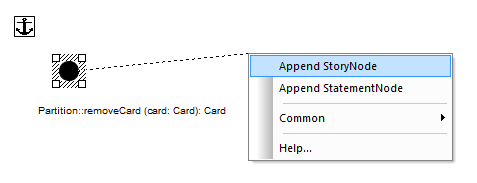
\includegraphics[width=0.8\textwidth]{ea_sdmQuickLinkStoryNode}
  \caption{Create new activity node}  
  \label{fig:sdm_new_activity_node}
\end{center}
\end{figure}

\item[$\blacktriangleright$] If you quick-created correctly, you should now have a start node, an activity node called \texttt{ActivityNode 1}, and an edge
connecting the two items. Complete the activity by quick creating a stop node as depicted in Fig.~\ref{fig:sdm_stop_node}.

\begin{figure}[htp]
\begin{center}
  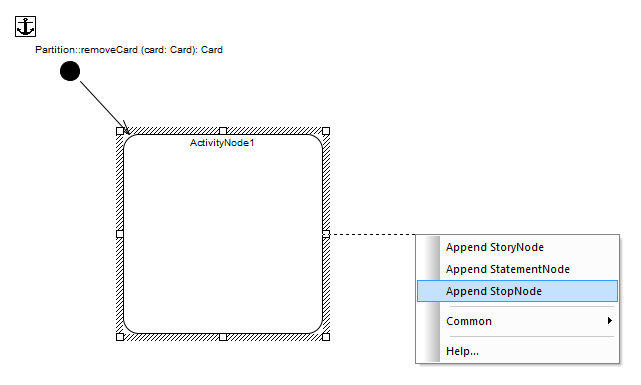
\includegraphics[width=\textwidth]{ea_sdmAppendStopNode}
  \caption{Complete activity with a stop node}  
  \label{fig:sdm_stop_node}
\end{center}
\end{figure}

\vspace{0.5cm}

\item[$\blacktriangleright$] If everything is correct, you should now have a complete activity that models the \emph{control flow} of the method. 
The semantics of our activity is pretty straightforward -- the control begins in the start node, and flows along edges and their connected activity nodes until
it reaches a stop node, where it finally terminates. 

\vspace{0.5cm}

\item[$\blacktriangleright$] While \emph{Stop Node} is pretty self explanitory, you may be wondering at this point about the differences between a \emph{story
node} and a \emph{statement node}. Since not all activity nodes can contain story patterns (i.e., start and stop nodes), those that can are called \emph{story
nodes}. Statement nodes .. we'll encounter these in a later SDM, but for now, lets finish our first story node.

\vspace{0.5cm}

\item[$\blacktriangleright$] To create the story pattern, double click \texttt{ActivityNode 1} to prompt the dialogue depicted in Fig.~\ref{fig:story_pattern}.

\begin{figure}[htpb]
\begin{center} 
  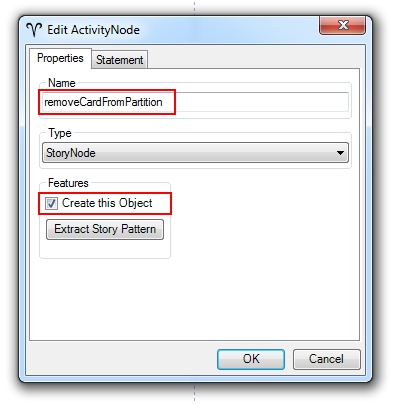
\includegraphics[width=0.6\textwidth]{ea_sdmEditActivityNode}
  \caption{Start modelling story pattern in activity node}  
  \label{fig:story_pattern}
\end{center}
\end{figure}

\vspace{0.5cm}

\item[$\blacktriangleright$] Enter `removeCardFromPartition' as the name of the story node, select \texttt{Create this Object}, and click \texttt{OK}. The
activity node now has a single \emph{object variable}, \texttt{this} (Fig.~\ref{fig:tool_box}).

\begin{figure}[htp]
\begin{center}
  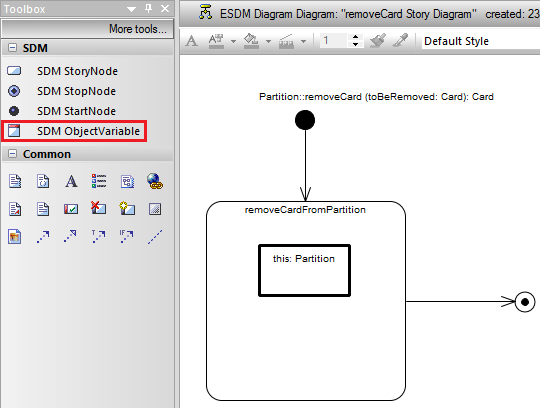
\includegraphics[width=0.8\textwidth]{ea_sdmNewObjVar}
  \caption{Add a new object variable from the toolbox}  
  \label{fig:tool_box}
\end{center}
\end{figure}

\newpage

\item[$\blacktriangleright$] To create an object variable that can be assigned to other objects, choose \texttt{SDM ObjectVariable} from the toolbox
(Fig.~\ref{fig:tool_box}), then click inside the activity node to raise the properties window for the new object (Fig.~\ref{fig:object_variable_properties}).

\vspace{0.5cm}

\begin{figure}[htp]
\begin{center}
  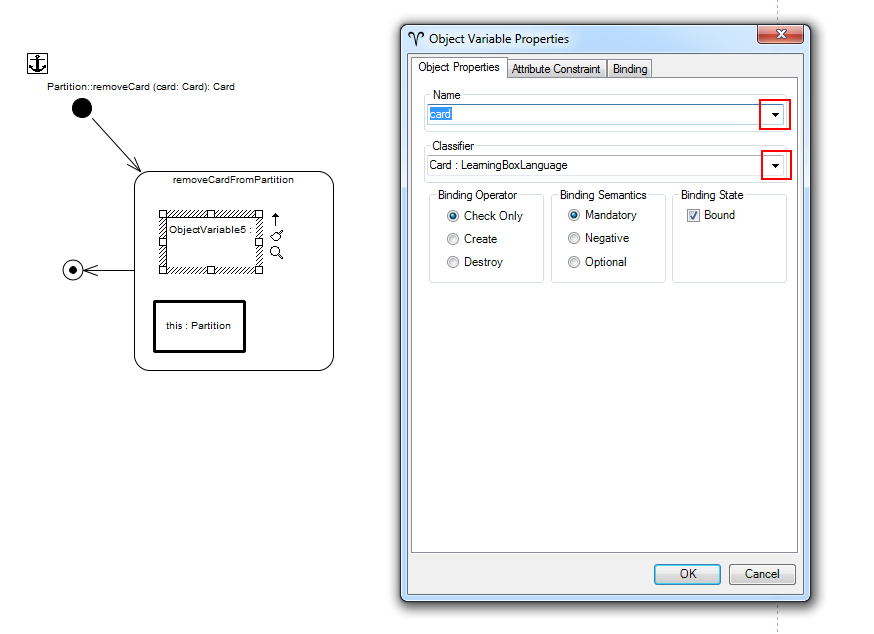
\includegraphics[width=\textwidth]{ea_sdmPropertiesObjVar}
  \caption{Specify properties of the added object variable}  
  \label{fig:object_variable_properties}
\end{center}
\end{figure}


\item[$\blacktriangleright$] Choose \texttt{card} as the name of the object variable and set \texttt{Card} as its type using the relevant drop-down menus.
Since \texttt{card} is a parameter of the method, it is offered as a possible name in the drop-down menu, which can be directly chosen to prevent annoying
typing mistakes.

\vspace{0.5cm}

\item[$\blacktriangleright$] In this dialogue, note that the \texttt{Bound} option must be set. We have now seen two cases in this activity for bound object
variables: the assignment to \texttt{this}, and an assignment to the parameter of the method.

\vspace{0.5cm}

\item[$\blacktriangleright$] To create a \emph{link variable} between the current partition (who invoked \texttt{removeCard}), and the
card to be removed (passed in as a parameter of \texttt{removeCard}), choose the object variable \texttt{this} and quick-link it to \texttt{card}
(Fig.~\ref{fig:link_variable}).

\begin{figure}[htpb]
\begin{center}
  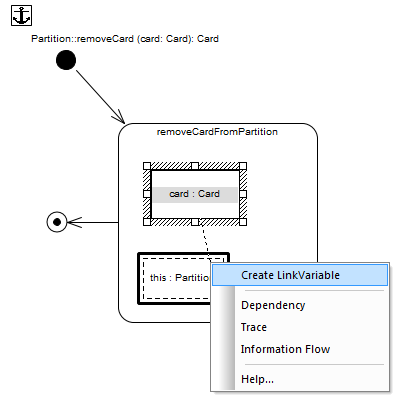
\includegraphics[width=0.6\textwidth]{ea_sdmCreateLinkVar}
  \caption{Create a link variable}   
  \label{fig:link_variable}
\end{center}
\end{figure}

\item[$\blacktriangleright$] According to the metamodel, there is only one possible link type between a partition and card. Select this and set the
\emph{Binding Operator} to \texttt{Destroy} (Fig.~\ref{fig:link_variable_properties}). 

\vspace{0.5cm}

% Had to force (h!) image to appear here; no other images were co-operating
\begin{figure}[h!]
\begin{center} 
 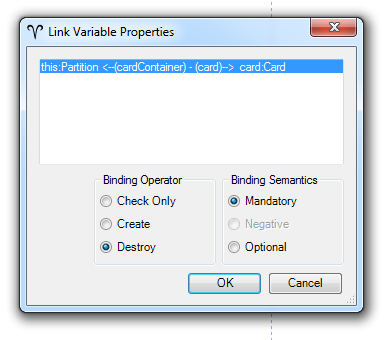
\includegraphics[width=0.6\textwidth]{ea_sdmBindLink}
  \caption{Specify properties for created link variable}  
  \label{fig:link_variable_properties}
\end{center}
\end{figure}

\vspace{0.5cm}

\item[$\blacktriangleright$] Remember how we said that this method should return the same card that was passed in? As luck would have it, a return value for any
SDM can be specified in the stop node. As depicted in Fig.~\ref{fig:stop_node_return_value}, double-click the stop node to prompt the \texttt{Edit StopNode} dialogue. 

\begin{figure}[htbp]
\begin{center}
  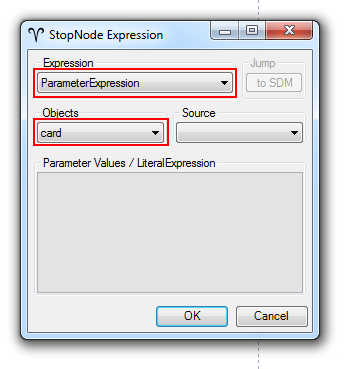
\includegraphics[width=0.5\textwidth]{ea_sdmStopNodeExpr}
  \caption{Adding a return value to the stop node}  
  \label{fig:stop_node_return_value}
\end{center}
\end{figure}

\item[$\blacktriangleright$] In the \texttt{Expression} field, choose \texttt{ParameterExpression} as the expression, and \texttt{card} as the parameter.

\vspace{0.5cm}

We're nearly done! As you can see, by using several different dialouges, eMoflon employs a simple context-sensitive expression language for specifying required
values. We have intentionally avoided creating a full-blown sub-language, and limit expressions to a few simple types.\footnote{We also do not support nesting
expressions} The philosophy here is to keep things simple and concentrate on what SDMs are good for -- expressing structural changes. Our approach is to
provide a clear and type-safe interface to a general purpose language (Java) and support a simple \emph{fallback} as soon as things get low-level and difficult
to express as a pattern.

The alternative approach to eMoflon would be to support arbitrary expressions, for example, in a script language like JavaScript or in an appropriate
DSL\footnote{A DSL is a Domain Specific Language: a language designed for a specific task which is usually simpler than a general purpose language like Java and
more suitable for the exact task.} designed for this purpose. In the following SDM implementations, we'll learn the other expression types eMoflon supports,
and how to use them. For the moment however, we'll use a \emph{ParameterExpression} which refers to the parameters of the current
method, exactly what we needed and have used for our \texttt{removeCard} SDM.

\item[$\blacktriangleright$] Returning to the activity, if you've done everything right, your complete SDM should now resemble
Fig.~\ref{fig:sdm_complete_control_flow}. The return value is indicated below the stop node.


\begin{figure}[htbp]
\begin{center}
  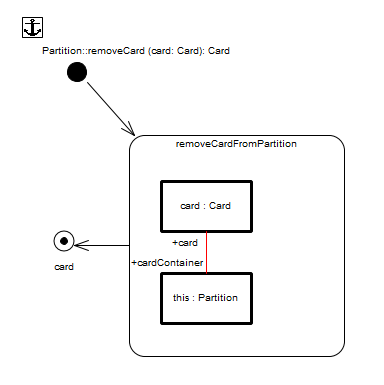
\includegraphics[width=0.7\textwidth]{ea_sdmRemoveComplete}
  \caption{Complete SDM for \texttt{Partition::removeCard}}  
  \label{fig:sdm_complete_control_flow}
\end{center}
\end{figure}

Let's take a step back and briefly review what we have specified:  if \texttt{p.remove\-Card(c)} is invoked for a partition \texttt{p}, with a card, \texttt{c},
as its argument, the specified pattern will \emph{match} only if that card is contained in the partition. After determining matches for all variables, the
link between the partition and the card is deleted, effectively ``removing'' the card from the partition. If the card is \emph{not} contained in the partition,
the pattern won't match, and nothing will happen. In both cases, the card that was passed in is returned.

\item[$\blacktriangleright$] Well, that's it! Congratulations! You have now specified your first complete SDM using eMolfon! Don't forget to save your
files, validate and export your pattern to the Eclipse workspace\footnote{Go to to ``\texttt{Extensions}" and select \texttt{Add-In Windows} to activate
eMoflon's console. If you're unsure how to validate, export, or use this window, review Part II, section 3}, then build your metamodel's code.

\item[$\blacktriangleright$] If you're unable to export or generate code successfully, compare your SDM carefully with Fig.~\ref{fig:sdm_complete_control_flow}
and make sure you haven't forgotten anything.

\item[$\blacktriangleright$] If successful, navigate to ``Learning\-Box\-Language/\-gen/\-Learning\-Box\-Language/\-impl/\-Partition\-Impl.java" to the
\texttt{\-remove\-Card} declaration. Inspect the generated implementation for your method. Notice all the null checks that are automatically created - only a
very conscientious (and probably slightly paranoid) programmer would program so defensively!

\item[$\blacktriangleright$] We admit, this section had a lot of reading and theory - it does get better! Soon, you'll be an eMoflon master, and we'll hardly
need to give you any instructions at all! In the following sections, we shall explore further features of SDM that allow for really expressive and powerful
patterns. If you'd like to see how this SDM is implemented in the textual syntax, check out Fig.~\ref{fig:deleteReference} in the next section.

\fancyfoot[R]{ $\triangleright$ \hyperlink{sec:checkCard}{Next} }

\end{itemize}

